%!TEX TS-program = xelatex
\documentclass[]{friggeri-cv}
\usepackage{afterpage}
\usepackage{hyperref}
\hypersetup{colorlinks=false,linkbordercolor=red,linkcolor=green,pdfborderstyle={/S/U/W 1}}

\usepackage{color}
\usepackage{xcolor}
\usepackage{smartdiagram}
\usepackage{fontspec}
% if you want to add fontawesome package
% you need to compile the tex file with LuaLaTeX
% References:
%   http://texdoc.net/texmf-dist/doc/latex/fontawesome/fontawesome.pdf
%   https://www.ctan.org/tex-archive/fonts/fontawesome?lang=en
%\usepackage{fontawesome}
\usepackage{metalogo}
\usepackage{dtklogos}
\usepackage[utf8]{inputenc}
\usepackage{tikz}
\usetikzlibrary{mindmap,shadows}
\hypersetup{
    %pdftitle={resume},
    %pdfauthor={sergio_mazucato},
    %pdfsubject={},
    %pdfkeywords={},
    colorlinks=false,           % no lik border color
    allbordercolors=white       % white border color for all
}

\newfontfamily\myfont[Ligatures=TeX]{Times New Roman}

\smartdiagramset{
    bubble center node font = \footnotesize,
    bubble node font = \footnotesize,
    % specifies the minimum size of the bubble center node
    bubble center node size = 0.5cm,
    %  specifies the minimum size of the bubbles
    bubble node size = 0.5cm,
    % specifies which is the distance among the bubble center node and the other bubbles
    distance center/other bubbles = 0.3cm,
    % sets the distance from the text to the border of the bubble center node
    distance text center bubble = 0.5cm,
    % set center bubble color
    bubble center node color = pblue,
    % define the list of colors usable in the diagram
    set color list = {lightgray, materialcyan, orange, green, materialorange, materialteal, materialamber, materialindigo, materialgreen, materiallime},
    % sets the opacity at which the bubbles are shown
    bubble fill opacity = 0.6,
    % sets the opacity at which the bubble text is shown
    bubble text opacity = 0.5,
}

\addbibresource{bibliography.bib}
\RequirePackage{xcolor}
\definecolor{pblue}{HTML}{0395DE}

\begin{document}
\header{Sergio}{Mazucato}
      {Electrical Engineer}
      
% Fake text to add separator      
\fcolorbox{white}{gray}{\parbox{\dimexpr\textwidth-2\fboxsep-2\fboxrule}{%
.....
}}

% In the aside, each new line forces a line break
\begin{aside}
  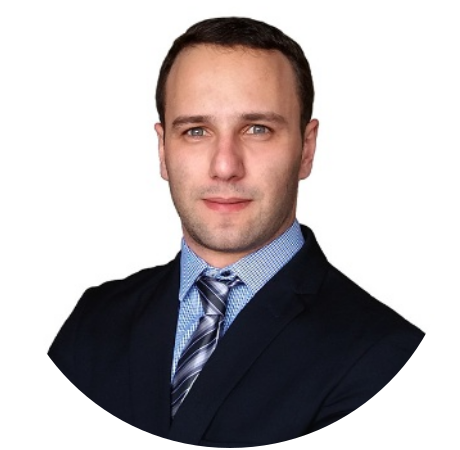
\includegraphics[scale=0.32]{img/linkedin_.png}
  \section{Contact}
    Rainäckerstr. 9
    Filderstadt, 70794
    Germany
    ~
    +49 171 844 0518
    \href{mailto:sergiomazucato@gmail.com}{\textbf{sergiomazucato@}\\gmail.com}
    ~
  \section{Web References}
    \href{https://www.linkedin.com/in/sergiomazucato/}{LinkedIn}
    \href{https://github.com/sergiomazucato}{GitHub}
    ~
  % use  \hspace{} or \vspace{} to change bubble size, if needed
	\section{Programming}
	    \textbf{Python}
\includegraphics[scale=0.38]{img/4bubbles.png}
	    \textbf{C}
\includegraphics[scale=0.38]{img/4bubbles.png}
	    \textbf{Matlab}
\includegraphics[scale=0.38]{img/5bubbles.png}
	    \textbf{Assembly}
\includegraphics[scale=0.38]{img/3bubbles.png}
	    ~
	\section{Languages}
	    \textbf{English}
\includegraphics[scale=0.40]{img/5stars.png}
	    \textbf{German}
\includegraphics[scale=0.40]{img/4stars.png}
	    \textbf{Italian}
\includegraphics[scale=0.40]{img/3stars.png}
	    \textbf{Portuguese}
\includegraphics[scale=0.40]{img/5stars.png}
	    ~
	\section{Places Lived}
		~
		
\includegraphics[scale=0.03]{img/brazil.png}    
\includegraphics[scale=0.03]{img/italy.png}   
\includegraphics[scale=0.03]{img/germany.png}
    	~
    \section{Appreciated Activities}
    	~
	    Problem solving 
\includegraphics[scale=0.40]{img/point.png}
	    Programming 
\includegraphics[scale=0.40]{img/point.png}
	    Electronics 
\includegraphics[scale=0.40]{img/point.png}
	    Math 
\includegraphics[scale=0.40]{img/point.png}
	    ~
\end{aside}
~
\section{Experience}
\begin{entrylist}
  \entry
    {09/17 - Now}
    {Technical Consultant}
    {\normalsize{Gemalto (Stuttgart)}}
    {As a Technical Consultant, Sergio is the thecnical responsible for the Smartcards Portfolio (chips for bank cards) of the financial sector. He is in charge of the \textbf{solution design},\textbf{ specification},\textbf{ development management},\textbf{ validation},\textbf{ delivery} and its\textbf{ maintenance}.\\ He is also the technical interface with customers for \textbf{presales} and \textbf{after sales} activities, being responsible for the \textbf{project valuation} in case of new implementations and technical support within the lifecycle of a product, as software troubleshooting on low and high-level programming languages.
     \\}
  \entry
    {08/16 - 08/17}
    {Technical Project Manager}
    {\normalsize{Gemalto (Sao Paulo)}}
    {As a technical project manager, he was responsible for the IT project management in Sao Paulo (Brazil) for the first tier accounts. The standard projects were Data Processing Software and Assembly-like scripts for Smartcards personalization. In this role, the common projects were treated over an \textbf{Agile} approach and the customized projects on a \textbf{PMP} standard.\\}
    \entry
    {08/15 - 08/16}
    {Project Engineer}
    {\normalsize{Gemalto (Sao Paulo)}}
    {As a technical account leader he was responsible for software development on high level (\textbf{javascript} and \textbf{Python}) and low level (\textbf{assembly}-like) languages, definition of the electrical profile of smartcards and advisory over chip's behavior for several customers. \\}
    \entry
    {02/15 - 07/15}
    {Electrical Engineer - Trainee Role}
    {\normalsize{Cocal Energia (Sao Paulo)}}
    {As part of the industrial management team, was deeply involved with the PMO and the electric power generation \& devices maintenance.
    \\}
    \entry
    {07/14 - 01/15}
    {Technical Consulting internship}
    {\normalsize{Gemalto (Sao Paulo)}}
    {Acted as part of the team responsible for 2nd tier of clients, representing 100k units of cards yearly. The role of the intern was to support the development of software projects and the consultants over the electrical specification of smartcards. \\}
    \entry
    {01/14 - 07/15}
    {Application Engineering internship}
    {\normalsize{Varixx electronics (Sao Paulo)}}
    {Acted as part of the team responsible for presales activities, the main task of the intern was to analyse the products (circuits) and to develop test-cases for the engineers. This role was also up to the redesign of electrical circuits and documentation update.\\}
\end{entrylist}
\newpage
\section{Education}
\begin{entrylist}
  \entry
    {2016 - 2016}
    {Specialization in Project Management}
    {Fundacao Getulio Vargas (FGV)}
    {}
  \entry
    {2010 - 2015}
    {Bachelor's degree in Electrical Engineering}
    {Federal University of Parana}
    {cGPR: 3.28 - Rated as \textbf{best} student of the university at the National Exam for the Assessment of Student Performance, the rank for all other comparisons as city, state and country are above p75 (between the best 25\%). \\}
  \entry
    {2013}
    {ERASMUS}
    {FH-Zwickau}
    {IEEE Industrial Electronics Society \textbf{Award} in recognition for a paper presented at IECON2013 in Vienna.}
\end{entrylist}

%

%\begin{aside}
%~
%~
%~
%  \section{OS Preference}
%    \textbf{GNU/Linux}
\includegraphics[scale=0.40]{img/5stars.png}
%    \textbf{Unix}
\includegraphics[scale=0.40]{img/4stars.png}
%    \textbf{MacOS}
\includegraphics[scale=0.40]{img/2stars.png}
%    \textbf{Windows}
\includegraphics[scale=0.40]{img/1stars.png}
%    ~
%\end{aside}

\section{Publications}

\href{http://dx.doi.org/10.4018/ijncr.2014010101}{
\includegraphics[height=\fontcharht\font`\B]{img/igi_global_.png} Automatic Tuning of PSSs and PODs Using a Parallel Differential Evolution Algorithm. In: \textbf{2014 International Journal of Natural Computing Research}, v. 4, p. 1-16, 2014}.\\
\\
\href{http://dx.doi.org/10.1109/IECON.2013.6699462}{
\includegraphics[scale=0.11]{img/ieee.jpg} Parallel Simultaneous and Coordinated Tuning of PSSs Using Ant Colony Optimization. In: \textbf{2013 IEEE Industrial Electronics Society}, 2013 Vienna, Austria.}\\
\\
\href{http://dx.doi.org/10.1109/IECON.2013.6699436}{
\includegraphics[scale=0.11]{img/ieee.jpg} Combining Subpopulation Tables, Non-dominated Solutions and Strength Pareto of MOEAs to treat Service Restoration Problem in Large-Scale Distribution Systems. In: 2013 \textbf{IEEE Industrial Electronics Society}, 2013 Vienna, Austria.}\\
\\
\href{http://dx.doi.org/10.1109/PESGM.2012.6345340}{
\includegraphics[scale=0.11]{img/ieee.jpg} Simultaneous and coordinated tuning of PSSs and PODs using differential evolution. In: 2012 \textbf{IEEE Power \& Energy Society General Meeting}, 2012, San Diego. 2012 IEEE Power and Energy Society General Meeting.}\\
\\
\section{Complementary Info}

\begin{itemize}
	\item Linux basic knowledge (10+ years of personal use).
	\item Volunteer work for three years at two College projects: \textit{"Evolutive algorithms applied to corporeal exercises of people in rehab"} and \textit{"Local factors and regional potentialities of the city Cornelio Procopio"}.
	\item Teacher assistent during one year for \textit{Electrical Machinery} and \textit{Electricity and Magnetism}.
	\item This document was generated \footnote{compiled on \today} with Python and \myfont{\LaTeX} \footnote{\url{https://github.com/sergiomazucato/resume}}.\\
\end{itemize}

%\begin{flushleft}
%\emph{\today}%May 8th, 2016}
%\end{flushleft}

\end{document}
